%%! program = pdflatex
%
%\documentclass[12pt,a4paper]{article} 
%%\usepackage{biblatex}
%%\usepackage{arc-dp}
%\usepackage{amssymb,amsfonts,latexsym}
%\newcommand{\MTNoLimits}[1]{\ensuremath{\mathop{#1}\nolimits}}
%\newcommand{\CL}[1]{\MTNoLimits{\mathcal{#1}}}
\newcommand{\SF}[1]{\mbox{\sf #1}}
\newcommand{\MT}[1]{\ensuremath{\mathop{#1}}}


% Sets
%\def\QProp{\CL{Q\!P}}
\def\QProp{\mathcal{Q\!P}}
\def\HAL{\mathcal{H}}
%\def\contains{\MT{\succcurlyeq}}
\def\contains{\MT{\succcurlyeq}}

\newcommand{\interference}{\ensuremath{\mathop{Intf}}}
\newcommand{\ket}[1]{\ensuremath{|#1\rangle}}
\newcommand{\bra}[1]{\ensuremath{\langle #1|}}
\newcommand{\scprod}[2]{\ensuremath{\langle #1 | #2 \rangle }}
\newcommand{\lprod}[2]{\ensuremath{\langle #1 | #2  }}
\newcommand{\rprod}[2]{\ensuremath{ #1 | #2 \rangle }}
\newcommand{\rv}[1]{\ensuremath{\mathbf{#1}}}
\newcommand{\projector}[1]{\ensuremath{\mathbf{#1}}}
\newcommand{\xpect}[3]{\ensuremath{\langle #1 | #2 | #3 \rangle}}
\newcommand{\colvec}[1]{
   \left ( \begin{array}{c}
              #1_1 \\
              \vdots \\
              #1_n
              \end{array}
    \right )
}
\newcommand{\lenvec}[1]{\ensuremath{\|#1\|}}
%\newcommand{\qed}{\hfill \ensuremath{\Box}}
\newcommand{\word}[1]{\emph{#1}}
\newcommand{\comment}[2]{
\vspace{8pt} \hrule \vspace{2pt}
\noindent {\sf \textbf{#1}: #2}
\vspace{2pt} \hrule \vspace{8pt} 
}
\newcommand{\tr}{\operatorname{tr}}
\newcommand{\oprod}[2]{\ensuremath{| #1 \rangle\langle #2 |}}


% \renewcommand{\comment}[2]{}

\newcommand{\inlinecomment}[2]{\fbox{\sf \textbf{#1}: #2}}

\newcommand\remove[1]{}



%\usepackage{amsfonts}
%\usepackage{amsmath}
%\usepackage{graphicx}
%\usepackage{times}
%\usepackage{setspace}
%\usepackage{fancyhdr}
%\usepackage{color}
%\usepackage[normalem]{ulem}
%\usepackage{subfig}
%\usepackage{float}
%\usepackage{caption}
%\usepackage{array}
%\usepackage{pgfgantt}
%\usepackage{url}
%\usepackage{enumitem}
%\usepackage{subfig}
%\usepackage{pgfgantt}
%\usepackage{wrapfig}
%\usepackage{enumitem}
%\usepackage[bottom]{footmisc}
%\usepackage{soul}
%\usepackage{pgfgantt}
%\usepackage{setspace}
%
%
%
%
%
%
%\usepackage[square,numbers]{natbib}
%\setlength{\bibsep}{0pt plus 0.3ex}
%\setlength{\parskip}{0pt}
%
%\usepackage{paralist}
%\renewenvironment{thebibliography}[1]{%
%\textsc{\textbf{}}
%\let\par\relax\let\newblock\relax%
%\inparaitem[{[}1{]}]}{\endinparaitem}
%
%
%\usepackage{etoolbox}
%\makeatletter
%\patchcmd{\@lbibitem}{\item[\hfil\NAT@anchor{#2}{\NAT@num}]}{\item[\NAT@anchor{#2}{\NAT@num}]}{}{}
%\makeatother
%
%
%
%
%
%
%
%
%%\usepackage[square,numbers]{natbib}
%%\setlength{\bibsep}{0pt plus 0.3ex}
%%\setlength{\parskip}{0pt}
%
%%\usepackage{bibspacing}
%%\setlength{\bibitemsep}{.2\baselineskip plus .05\baselineskip minus .05\baselineskip}
%
%%\usepackage{biblatex}
%%\defbibenvironment{bibliography}
%%  {}
%%  {}
%%  {\addspace
%%   \printtext[labelnumberwidth]{%
%%     \printfield{prefixnumber}%
%%     \printfield{labelnumber}}%
%%   \addhighpenspace}
%
%%\usepackage{filecontents}
%
%%\usepackage{biblatex}
%%\defbibenvironment{bibliography}
%%  {}
%%  {}
%%  {\addspace
%%   \printtext[labelnumberwidth]{%
%%     \printfield{prefixnumber}%
%%     \printfield{labelnumber}}%
%%   \addhighpenspace}
%
%
%
%%%%%% cut here
%%
%%\usepackage{paralist}
%%
%%%\setlength\labelsep{.0em}
%%%\setlength\itemsep{0pt plus 0.3ex}
%%%\setlength\parsep{0pt plus 0.3ex}
%%  \setlength{\parskip}{0pt}
%%  \setlength{\itemsep}{0pt plus 0.3ex}
%%%\setlength\labelwidth{.0em}
%%%\setlength\leftmargin{.0em}
%%
%%\makeatletter
%%\renewenvironment{thebibliography}[1]
%%     {\section*{\refname}%
%%      \@mkboth{\MakeUppercase\refname}{\MakeUppercase\refname}%
%%      \begin{inparaenum}%
%%      \list{\@biblabel{\@arabic\c@enumiv}}%
%%           {\settowidth\labelwidth{\@biblabel{#1}}%
%%            \leftmargin\z@
%%            \advance\leftmargin\z@
%%            \@openbib@code
%%            \usecounter{enumiv}%
%%            \let\p@enumiv\@empty
%%            \renewcommand\theenumiv{\@arabic\c@enumiv}}%
%%%      \sloppy
%%      \clubpenalty4000
%%      \@clubpenalty \clubpenalty
%%      \widowpenalty4000%
%%      \sfcode`\.\@m}
%%     {\def\@noitemerr
%%       {\@latex@warning{Empty `thebibliography' environment}}%
%%      \endlist\end{inparaenum}}
%%\renewcommand\newblock{}
%%\makeatother
%%
%%%%%% cut here 
%
%%% ADD THE FOLLOWING COUPLE LINES INTO YOUR PREAMBLE
%%\let\OLDthebibliography\thebibliography
%%\renewcommand\thebibliography[1]{
%%  \OLDthebibliography{#1}
%%  \setlength{\parskip}{0pt}
%%  \setlength{\itemsep}{0pt plus 0.3ex}
%%}
%
%%\let\oldthebibliography=\thebibliography
%%  \let\endoldthebibliography=\endthebibliography
%%  \renewenvironment{thebibliography}[1]{%
%%    \begin{oldthebibliography}{#1}%
%%      \setlength{\parskip}{0ex}%
%%      \setlength{\itemsep}{0ex}%
%%  }%
%%  {%
%%    \end{oldthebibliography}%
%%  }
%
%
%\usepackage{booktabs} % for spacing tables
%\usepackage{tabularx} % auto table sizing
%\usepackage{multirow} % table multirow
%
%%\usepackage{epsf}
%%\usepackage{fancyheadings}
%%\usepackage{subfigure}
%%\usepackage{pst-gantt}
%%\usepackage{tweaklist}
%
%\newcolumntype{L}[1]{>{\raggedright\let\newline\\\arraybackslash\hspace{0pt}}m{#1}}
%\newcolumntype{C}[1]{>{\centering\let\newline\\\arraybackslash\hspace{0pt}}m{#1}}
%\newcolumntype{R}[1]{>{\raggedleft\let\newline\\\arraybackslash\hspace{0pt}}m{#1}}
%
%%\let\OLDthebibliography\thebibliography
%%\renewcommand\thebibliography[1]{
%%  \OLDthebibliography{#1}
%%  \setlength{\parskip}{1pt}
%%  \setlength{\itemsep}{1pt plus 0.3ex}
%%}
%
%\newcommand{\hlg}[2][green]{{%
%	\colorlet{foo}{#1}%
%	\sethlcolor{foo}\hl{#2}}%
%}
%
%\newcommand{\hly}[2][yellow]{{%
%	\colorlet{foo}{#1}%
%	\sethlcolor{foo}\hl{#2}}%
%}
%
%\newcommand{\hlr}[2][red]{{%
%	\colorlet{foo}{#1}%
%	\sethlcolor{foo}\hl{#2}}%
%}
%
%\newcommand{\hlo}[2][orange]{{%
%	\colorlet{foo}{#1}%
%	\sethlcolor{foo}\hl{#2}}%
%}
%
%
%%\renewcommand{\enumhook}{\setlength{\topsep}{0pt}%
% % \setlength{\itemsep}{-2mm}}
%%\renewcommand{\itemhook}{\setlength{\topsep}{0pt}%
%%  \setlength{\itemsep}{-2mm}}
%  %%%%%UNCOMMENT THE NEXT COMMAND IF NEEDED
%%\renewcommand{\descripthook}{\setlength{\topsep}{0pt}%
%%  \setlength{\itemsep}{-2mm}}
%
%%\pagestyle{fancy}
%
%%\input{psfig.sty}
%\newcommand{\todo}[1]{\textcolor{red}{#1}}
%\newcommand{\rules}[1]{\textcolor{blue}{#1}}
%\newcommand{\pset}{ {\rm P} \! \! \! {\rm P} }
%\date{}
%%\include{psfig}
%\remove{
%\topmargin -15mm
%\headheight 0pt
%\headsep 0pt
%\textheight 285mm
%\oddsidemargin -15mm
%\evensidemargin -15mm
%\textwidth 190mm
%\columnsep 10mm
%\marginparwidth 0pt
%\marginparsep 0pt
%}
%
%\usepackage[top=0.5cm, bottom=0.5cm, left=0.5cm, right=0.5cm]{geometry}
%\parindent=4mm
%\parskip=0.2mm
%
%%\usepackage{geometry} % see geometry.pdf on how to lay out the page. There's lots.
%%\geometry{a4paper} % or letter or a5paper or ... etc
%% \geometry{landscape} % rotated page geometry
%
%
%%\linespread{1.5}
%
%\newcommand*{\TitleFont}{%
%      \usefont{\encodingdefault}{\rmdefault}{b}{n}%
%      \fontsize{12}{12}%
%      \selectfont}
%
%%\title{Maximising cooling through urban planning using blue-green infrastructure}
%%\author{}
%\date{} % delete this line to display the current date
%
%%%% BEGIN DOCUMENT
%\begin{document}
%\rmfamily
%\date{}

\noindent \textbf{PROJECT TITLE: }\\ \noindent Urban heat mitigation through blue-green infrastructure

\subsection*{\TitleFont PROJECT AIMS AND BACKGROUND}

%Briefly outline the aims and provide the background of this application.
%Include information about national and international progress in this field of research and its relationship to this application.
%Refer only to research outputs that are accessible to the national and international
%research communities.


Extreme heat events cause more deaths in Australia than any other natural hazard\cite{Coates2014}, with risk disproportionately borne by the elderly and the very young\cite{Nicholls2008}. Future climate projections warn of more frequent, severe, and long-lasting heatwaves\cite{IPCC2013a} and exposure to dangerous levels of heat stress increasing by a factor of 5-10 by 2080\cite{Coffel2018}. Risks are further multiplied by the design of cities\cite{Coutts2012,Martilli2020} that result in increased heat loads in urban areas. Urban energy balances have been altered in several ways\cite{Oke1982}. These include anthropogenic heat from buildings and transport and reduced shading through diminishing tree canopy cover resulting in larger amounts of net energy at street level. Meanwhile, the conversion of vegetated to impervious surfaces and reductions of available water in cities shift the urban energy balance away from latent heat (water evaporation) towards increased sensible heat (heat that can be felt) and heat storage in urban surfaces. 

Strategies, especially those that utilise blue-green infrastructure (BGI)\cite{Norton2015,Bowler2010,Gunawardena2017,Newton2020} such as increased vegetation cover, water features, and water practices (rain gardens, misting systems, or pavement watering), are available to mitigate heat. These strategies are ideally considered during the planning of future development, before these decisions are hardened into the built form for decades to come. Benefits can also be realised by an analysis of existing areas to find problem areas and incorporating BGI through remedial redesign. Both cases are best addressed using modelling tools, but as will be detailed below, these tools are currently insufficient for this task. Compounding this, is that observational data on urban cooling through BGI, data essential for designing and testing the modelling tools, is very limited. In a systematic review of studies quantifying the cooling potential of irrigating urban green spaces \cite{Cheung2021}, only 19 studies were found, where only seven reported irrigation amounts and the majority were modelling studies or agricultural (and not specifically urban). \textbf{This leads to two project aims. The first is to perform a wide range of observations on BGI features, to quantify their cooling impacts and to uncover the mechanisms, patterns, and magnitudes behind the cooling. The second is to utilise these observations to improve existing models so that they are suitable to model a full range of BGI features and their human thermal comfort benefits. As a result, this project will provide high value tools to a wide range of users including future researchers, consultants, and urban planners, enabling them to analyse and redesign urban areas to maximise the cooling benefits of BGI.}

The use of water and vegetation has long been recognised as an effective method to mitigate urban temperature extremes \cite{Coutts2012,Bowler2010}, but as Gao \& Santamouris \cite{Gao2019} find, some research exists on irrigation-induced temperature reductions in agriculture, but studies in urban areas are quite rare and at very early research stages. Agricultural studies can provide valuable insights but cannot capture the complexity of highly heterogeneous urban environments. A lack of high resolution measurements of temperature reductions and cooling mechanisms from irrigation leads to inconsistencies in expected cooling magnitudes between studies and uncertainties in the amounts of water required and optimal strategies to maximise cooling benefits. These gaps have an impact on our understanding of the general principles behind these methods of cooling. They have a large impact on model development. The lack of observations stands in the way of the design and validation of modelling tools. To fully incorporate urban cooling strategy into urban planning requires modelling tools that can account for the influences of BGI on human thermal comfort in cities. Further, to capture all the influences of urban geometry and materials on human thermal comfort, especially the influences on mean radiant temperature\cite{Kantor2011} (a temperature that accounts for the thermal stresses on a person from both solar exposure and energy/heat radiating from nearby surfaces), modelling needs to be done at a micro-scale (that is, at a grid square or pixel resolution under 1km). 

There are many urban models, however there are few modelling options available at an appropriate scale, that can account for all the elements of vegetation impacts and urban hydrology, and that can explicitly calculate parameters needed to calculate human thermal comfort. Some of the available urban models include ENVI-met\cite{Bruse1999}, VTUF-3D\cite{Nice2018a}, SOLWEIG/UMEP\cite{Lindberg2018}, PALM\cite{Dominik2019}, canyon air temperature (CAT)\cite{Erell2006}, and OTC3D\cite{Nazarian2018}. Other models offer lower resolution local-scaled (grid resolution greater than 1km) modelling (TARGET\cite{Broadbent2019c} and SURFEX\cite{Masson2013}) or of a single point averaged across an entire (often idealised) urban canyon (TEB\cite{Masson2002a},  TEB-Veg and TEB-Tree\cite{Lemonsu2012,Redon2020}, RayMan\cite{Matzarakis2010}/SkyHelios\cite{Matzarakis2011}, and Urban Tethys-Chloris (UT\&C)\cite{Meili2020}). Some of these models (e.g. ENVI-met, PALM) are highly spatially explicit at the cost of high computational burden (and in the case of ENVI-met high licensing costs), or high levels of configuration and software expertise (e.g. SURFEX requires modification and compilation of FORTRAN code). Others (e.g. UT\&C) rely on simplified parameterisations and an idealised representation of vegetation and urban canyons for producing a detailed time series of the energy balance at the local scale. 

Table \ref{tab:modelcompare} presents a comparison of available micro- and local-scaled urban models. Characteristics that are essential for human thermal comfort assessments of BGI are highlighted in green. They should be micro-scaled and provide high spatial resolution. Some models only output a single point, either a single location or one averaged across the entire area.  Local scaled modelling provides some insights but there are limitations to the level of understanding they can provide into the factors influencing urban heat. These and other limiting model characteristics are highlighted with orange. Major limitations in modelling BGI are highlighted in red. Ideally, the entire soil/plant/atmosphere continuum must be accounted for in detail, including vegetation and vegetated surfaces, hydrology/water balances, and latent energy fluxes (i.e. the energy due to water evaporation). High computational demand of some models also proves a limitation both for short-term simulations but especially for long-term simulations, which are required to understand the timing between mitigation strategies and extreme heat days. Some characteristics are highlighted in yellow, features that will be useful in modelling the full range of BGI features and some practices intended to reduce thermal stress during heat events (e.g. misting, watering green areas, or pavement-watering). Finally, assessing human thermal comfort requires the ability to predict mean radiant temperatures.

\begin{table}
\begin{tabular}{c c c c c c c c c c c}
\hline
Model & Scale & Spatial & Intensity & Veg. & Temp. & Geometry & Fluxes & Wind  & Hydrology  \\ \hline
ENVI-met\cite{Bruse1999}  &\hlg{M}&\hlg{M}&\hlr{H}&\hlg{F}&A,S,\hlg{M},\hlg{U}&\hlg{C}&\hlg{All}&\hly{C}&\hlg{W},\hlg{C},\hlg{m},\hly{M},\hly{G},\hlg{E},\hlg{P}\\
SOLWEIG\cite{Lindberg2018}   &\hlg{M}&\hlg{M} &\hlg{M}&S &\hlg{M}&\hlg{C}&K,L&N&\hlr{N}\\
PALM\cite{Dominik2019}      &\hlg{M}&\hlg{M} &\hlr{H}&\hlg{F} &A,S,\hlg{M},\hlg{U}&\hlg{C}&\hlg{All}&\hly{C}&\hlg{W},\hlg{C},\hlg{m},\hlg{E},\hlg{P}\\
OTC3D\cite{Nazarian2018}     &\hlg{M}&\hlg{M} &\hlg{M}&\hlr{N} &    \hlg{M},\hlg{U}&\hlg{C}&N,H,\hlg{E},K,G&E&\hlr{N}\\
SURFEX\cite{Masson2013}   &\hlo{L}&\hlg{M} &\hlg{M}&I &    A,\hlg{U}&I&\hlg{All}&R&\hlg{W},\hlg{C},\hlg{m},\hlg{E},\hlg{P}\\
TEB\cite{Masson2002a,Lemonsu2012,Redon2020}       &\hlo{L}&\hlo{S} &\hlg{M}&I & A,S   &I&\hlg{All}&R&\hlg{W},\hlg{C},\hlg{m},\hlg{E},\hlg{P}\\
RayMan\cite{Matzarakis2010}    &\hlg{M}&\hlo{S} &\hlg{L}&S &    \hlg{M}  &\hlg{C}& K,L &N&\hlr{N}\\
SkyHelios\cite{Matzarakis2011} &\hlg{M}&\hlo{Se}&\hlg{L}&S &    \hlg{M}  &\hlg{C}& K,L &N&\hlr{N}\\
UT\&C\cite{Meili2020}     &\hlo{L}&\hlo{S} &\hlg{M}&\hlg{F} &A,S    &I&\hlg{All}&R&\hlg{W},\hlg{C},\hlg{m},\hlg{E},\hlg{P}\\
SUEWS\cite{Jarvi2011}   &\hlo{L}&\hlo{S} &\hlg{L}&I & A,S,So  &I&\hlg{All}&N&\hlg{W},\hlg{C},\hlg{m},\hlg{E},\hlg{P}\\
BEP-Tree\cite{Krayenhoff2014a}  &\hlo{L}&\hlo{S} &\hlg{M}&I &A      &I&\hlg{All}&N&\hlr{N}\\
CAT\cite{Erell2006}       &\hlg{M}&\hlo{S} &\hlg{L}&\hlr{N} &A      &I&\hlg{All}&N&\hlr{N}\\ \hline
VTUF-3D\cite{Nice2018a}&\hlg{M}&\hlg{M} &\hlg{M}&\hlg{F} &A,S,\hlg{M},\hlg{U}&\hlg{C}&N,H,\hlg{E},K,L,G&R&\hlo{S},\hlg{m},\hlg{E} \\
TARGET\cite{Broadbent2019c} &\hlo{L}&\hlg{M} &\hlg{L}&I &A,S,\hlg{M},\hlg{U}&I&N,H,\hlg{E},K,L,G&R&\hlg{W},\hlo{S} \\ \hline
VTUF-3D v2&\hlg{M}&\hlg{M} &\hlg{M}&\hlg{F} &A,S,\hlg{M},\hlg{U}&\hlg{C}&\hlg{All}&R,\hly{A}&\hlg{W},\hlg{C},\hlg{m},\hly{M},\hly{G},\hlg{E},\hlg{P} \\
TARGET v2 &\hlo{L}&\hlg{M} &\hlg{L}&I &A,S,\hlg{M},\hlg{U}&I&\hlg{All}&R,\hly{A}&\hlg{W},\hlg{C},\hlg{m},\hly{M},\hly{G},\hlg{E},\hlg{P} \\
\hline

\end{tabular}
\caption{\label{tab:modelcompare}Comparison of micro and local-scale models, features, and limitations around modelling human thermal comfort and BGI. Modelling scale [\textbf{M}icro/\textbf{L}ocal], Spatial resolution [\textbf{S}ingle point/\textbf{Se}ries of points/\textbf{M}any points], Computational intensity [\textbf{L}ow/\textbf{M}edium/\textbf{H}igh], Vegetation [\textbf{F}ully modelled/\textbf{S}hape only/\textbf{I}dealised modelling/\textbf{N}ot modelled], Temperatures [\textbf{A}ir temperature, $T_{a}$/\textbf{S}urface temperature, $T_{surf}$/\textbf{M}ean radiant temperature,$T_{mrt}$,\textbf{U}TCI/\textbf{So}il temperature,$T_{soil}$], Urban geometry [\textbf{C}omplex/\textbf{S}imple/\textbf{I}dealised], Fluxes [\textbf{N}et/Sensible (\textbf{H})/Latent(\textbf{E})/Shortwave(\textbf{K})/\textbf{L}ongwave/\textbf{G}round storage/Anthropogenic(\textbf{F})/\textbf{All}(includes N,H,E,K,L,G,F)], Wind [\textbf{C}FD/\textbf{E}xternal CFD/\textbf{R}oughness calculations/\textbf{A}dvection/\textbf{N}one], Hydrology [\textbf{W}ater bodies/\textbf{S}imple irrigation/\textbf{C}omplex irrigation/Soil \textbf{m}oisture/\textbf{M}isting/\textbf{G}reen wall/\textbf{E}vapotranspiration/\textbf{P}recipitation/\textbf{N}one]. Green highlights indicate necessary model characteristics for BGI and HTC modelling. Yellow highlights indicate useful characteristics. Orange highlights indicate some limitations. Red highlights indicate difficult characteristics.}
\end{table}

To produce low to medium computational intensity models that are also able to account for the full range of BGI will require some enhancements to existing models. But addressing the limitations in these current modelling tools are hampered by a lack of comprehensive observations to enable model development and validations. Datasets to validate modelling techniques to model the entire soil / plant / atmosphere continuum are scarce\cite{Pataki2013}, particularly observational data related to urban greening and especially at a micro-scale and that account for heat and energy fluxes under a wide range of irrigation scenarios. In addition, no datasets to validate the micro-scaled variations of spatial and temporal distribution of heat and cooling at a neighbourhood scale providing detailed statistics about the amounts, times, and locations of outside water usage (i.e. which household, how many litres used to irrigate, and what hour of the day) are available. Most research around the cooling benefits of irrigation has been conducted through modelling studies\cite{Kanamaru2008,Yang2015a,Broadbent2018a}. There are very few observation-based irrigation studies that focus on urban areas\cite{Broadbent2017a}. Some agricultural observation-based studies of irrigation\cite{Chen2018b} can provide insights to irrigated urban green areas but lack the complex heterogeneity of urban areas. This scarcity of observations limits our understanding of the full benefits of BGI and without these quite specialised datasets, ensuring that modelling tools accurately reproduce the underlying mechanisms of cooling using BGI becomes challenging. Without suitable tools, it will be difficult to explore the full range of benefits BGI can provide and provide these in a form that urban designers and planners can use to minimise the impacts of their designs on urban heat and heat stress, and ultimately translate this knowledge and provide simplified tools to allow them to explore their designs iteratively during their planning processes. Because of many of these challenges, consultants working for designers and planners have rarely been able to utilise climate knowledge in urban planning\cite{Elasson2000} and the complexities of urban climate have complicated the communication of results\cite{Oke2006}. \textbf{This is the major problem that this project aims to address through a focused collection of observations of BGI features that will be used to upgrade modelling tools that can be used to fully explore the utilisation of BGI as an effective urban cooling strategy.}

\subsection*{\TitleFont INVESTIGATOR/CAPABILITY}

%Describe the:
%- Research Opportunity and Performance Evidence (ROPE) including record of high
%  quality research outputs appropriate to the discipline/s.
%- capability of candidate to build collaborations both within Australia and    internationally.

During my PhD, I developed the Vegetated Temperature of Urban Facets in 3-D (VTUF-3D)\cite{Nice2018a} urban micro-climate model to examine the human thermal comfort impacts of street trees and water features (i.e. BGI). Immediately following, I co-developed The Air-temperature Response to Greenblue-infrastructure Evaluation Tool (TARGET)\cite{Broadbent2019c} (with Asst Research Prof. Ashley Broadbent and others), Urban Tethys-Chloris (UT\&C)\cite{Meili2020} (with Meili Naika and others), and the Monash Simple Climate Model\cite{Dommenget2019} (MSCM) (with A/Prof. Dietmar Dommenget). I have used SOLWEIG / UMEP\cite{Lindberg2018} and TARGET for many thermal comfort modelling consulting projects. VTUF-3D is one of the few models currently available to examine the human thermal comfort impacts of BGI at a micro-climate scale. The source code for VTUF-3D, and my other local-scaled model TARGET, is freely available and currently being used by a number of other urban climate scientists (and consulting groups such as Alluvium\cite{MosiacInsights2020} and Marsden Jacob) around the world. 

I have published my model development work\cite{Nice2018a,Broadbent2019c,Meili2020,Dommenget2019} in the Q1 journals, Geoscientific Model Development (SJR Q1 3.238) and Urban Climate (SJR Q1 1.151). These publications demonstrate my range of expertise in designing and using local and micro-scale models, models that account for urban surface energy balances and the influence of BGI and the processes of urban hydrology and vegetation physiology. I have conducted research using micro-climate modelling to evaluate human thermal comfort benefits of urban vegetation and water and the use of urban morphology databases (such as WUDAPT) in urban heat modelling are represented in conference presentations\cite{Gal2020,Nice2020b} as well as a fully-refereed conference paper\cite{Todorovic2019a}. I am also currently participating in a consulting consortium for the Australian Department of Agriculture, Water and the Environment (DAWES) with Prof. Nigel Tapper (Monash) with Dr. Andrew Coutts, and Dr. Matthias Demuzere (RUB) utilising the TARGET model to examine health cost impacts of urban heat under future climate scenarios. I am currently collaborating with Aldo Rojas Mondaca from the Pontificia Universidad Cat\'{o}lica de Chile to add green roofs and green walls to VTUF-3D.

Through my participation in the CRC for Water Sensitive Cities across its 8 year research program (as well as the precursor project `Cities as Water Supply Catchments'), I have developed working relationships with many local and state governments as well as industry partners, in particular, water companies. Currently, I have two PhD students engaged in research in conjunction with South East Water in Melbourne and South Australia Water in Adelaide. In the first project, the Aquarevo housing estate\cite{SEW2020} is the site of a number of campaigns to make micro-climate observations (temperatures, humidity, radiation fluxes, wind, and soil moisture and temperatures) of various irrigation strategies as well as the energy balances of misting systems, resulting in one publication \cite{Cheung2021} so far. A second trial through South Australia Water has been examining the cooling benefits of irrigation at the Adelaide Airport\cite{CRCWCS2018,Ingleton2020,Qian2020}. This project will build on this work and collect more data in future observation campaigns, especially examining irrigation of a variety of surface types and the cooling benefits of irrigation at a precinct level.

I developed a method through a collaboration with Ariane Middel at Arizona State University and supervised research projects by Master's of IT students using neural networks and computer vision techniques to accurately detect sky pixels in outdoor imagery (and therefore calculate sky view factors from these images). This research was published as an invited first author submission\cite{Nice2020} in the Urban Climate journal. My use of urban morphology databases to generate local climate zones (LCZ) through a collaboration with Dr Negin Nazarian, A/Prof Melissa Hart, and Dr Mathew Lipson at UNSW have resulted in an AURIN grant application as well as a number of in-preparation articles.

My research has evolved beyond urban climates to provide expertise in additional areas, incorporating other types of urban modelling, and using neural networks and computer vision methods to utilise large imagery data sets. This work involves developing urban and neighbourhood typologies and to cluster similar urban areas based on their urban properties and by health and well-being outcomes. Two of these were published in Q1 journals\cite{Thompson2020,Wijnands2019} (SJR Q1 4.205 and SJR Q1 1.65) as well as \cite{Nice2020a}. This expertise will directly contribute to this project in creating more efficient urban models through identification of urban areas with similar morphology properties and clustering them based on similar urban heat thermal performance responses.

Before returning to university to complete a Master's degree and PhD, I had a 13 year career as a senior level software engineer, working predominately with C++ and Java (the Java 2 Enterprise Edition). The experience I gained in software design, development, and project management, to create and implement both the user interfaces and the backend functionality for complex business process flows has proven to be highly transferable to climate model development and a research career. 

Over the last few years, I have quickly developed a sizeable network of Australian and international collaborators. Through my urban climate network, I am currently working with members of the Urban Climate Research Center at Arizona State University, including Asst. Prof. Ariane Middel (specialising in urban heat) and Asst. Research Prof. Ashley Broadbent (urban climate modelling) and Naika Meili (urban ecohydrology) at ETH Zurich and have published 3 papers with them. I am participating, as a developer of two models, in Urban Plumber (multi-site model evaluation project, the next iteration of the Grimmond et al.\cite{Grimmond2011} intercomparison project) led by Mat Lipson (UNSW), Sue Grimmond (Reading) and Martin Best (UK Met Office). These intercomparision projects have been important periodic evaluations of the current state of the art in urban modelling and are led by some of the most important figures and research organisations in the urban climate field. 

I am an active participant in the UNSW Urban Climate group which forms one of the major research groups within the ARC Centre of Excellence for Climate Extremes. I am currently serving on the Early Career Researcher Engagement Committee for the upcoming 2023 International Conference on Urban Climate (ICUC-11) in Sydney, Australia with a number of other international ECR urban climate scientists. My frequent attendance at past International Conferences on Urban Climate (ICUC) strengthens my urban climate relationships and has enabled forming new collaborations. In public health and computer vision, I have been collaborating with Dr. James Woodcock (leading public health modelling in the MRC Epidemiology Unit at Cambridge) and Dr. Rahul Goel from Cambridge University. I am a co-investigator in a NHMRC/UKRI awarded grant partnership with Queen's University Belfast. Finally, I am an investigator on a Swiss National Science Foundation grant along with Dr. Jo\~{a}o Leit\~{a}o and Dr. Peter Bach from Eawag (the Swiss Federal Institute of Aquatic Science and Technology), using TARGET to model urban heat mitigation through stormwater infrastructure. Together, these collaborations connect me to a wide range of expertise across urban climates, climate modelling, urban hydrology, and public health and public health modelling.

In addition to the skills and relationships I bring to this project, my research lab, the Transport, Health and Urban Design Research Lab (THUD) at the University of Melbourne, strongly supports my independent research under the umbrella of urban design and public health. This project provides a unique opportunity to integrate the issue of urban heat and how to create better urban design to mitigate its impacts as a major research area into the lab's areas of expertise.

\subsection*{\TitleFont PROJECT QUALITY AND INNOVATION}

%Describe the:
%- contribution to an important gap in knowledge or significant problem;
%- novelty/originality and innovation of the proposed research (including any new
%methods, technologies, theories or ideas that will be developed);
%- clarity of the hypothesis, theories and research questions;
%- cohesiveness of the project design and implementation plan (including the
%appropriateness of the aim, conceptual framework, method, data and/or analyses);
%and
%- extent to which the research has the potential to enhance international collaboration.


Urban planners have access to a wide range of tools to assess their designs across many factors, but a lack of accessible tools to examine urban heat or the ability to integrate heat modelling into their normal processes means that cities will continue to grow larger and denser with little to no consideration to human thermal comfort and urban heat mitigation; urban heat health impacts will be locked in for decades to come. In addition, the lack of tools also hampers the analysis of existing areas for locations of high vulnerability and to allow the planning of effective emergency response plans. Testing urban heat mitigation strategies, especially those using BGI features, requires modelling tools that can resolve at a micro-scale the processes driving thermal comfort and be shown suitable to model impacts of BGI, the full soil/plant/atmosphere continuum. Common questions include what locations and which types of vegetation deliver the highest benefits, how much irrigation is needed, or what are the impacts of different types of surfaces. But first to ensure these tools can be made available, more fundamental research needs to be completed, that is high-resolution observations of BGI features to provide the datasets needed to design and test modelling tools. 


This project will be delivered through five work packages. These work packages include local and micro-climate \textbf{observations} of BGI, upgrading \textbf{models} to make them suitable for HTC assessments of BGI, a \textbf{co-design} process with industry partners and urban climatologists of the \textbf{scenario} analysis process to design scenarios of the greatest value to them, and a \textbf{dissemination} process to output the results back through the industry partners (reports and workshops) in addition to the traditional scientific channels (journals and conferences) and plan the next steps for the research to allow widespread adoption of these tools and insights. The overall structure of the project is shown in Figure \ref{fig:overall}.


\begin{figure}[ht]
\begin{center}
\fbox{
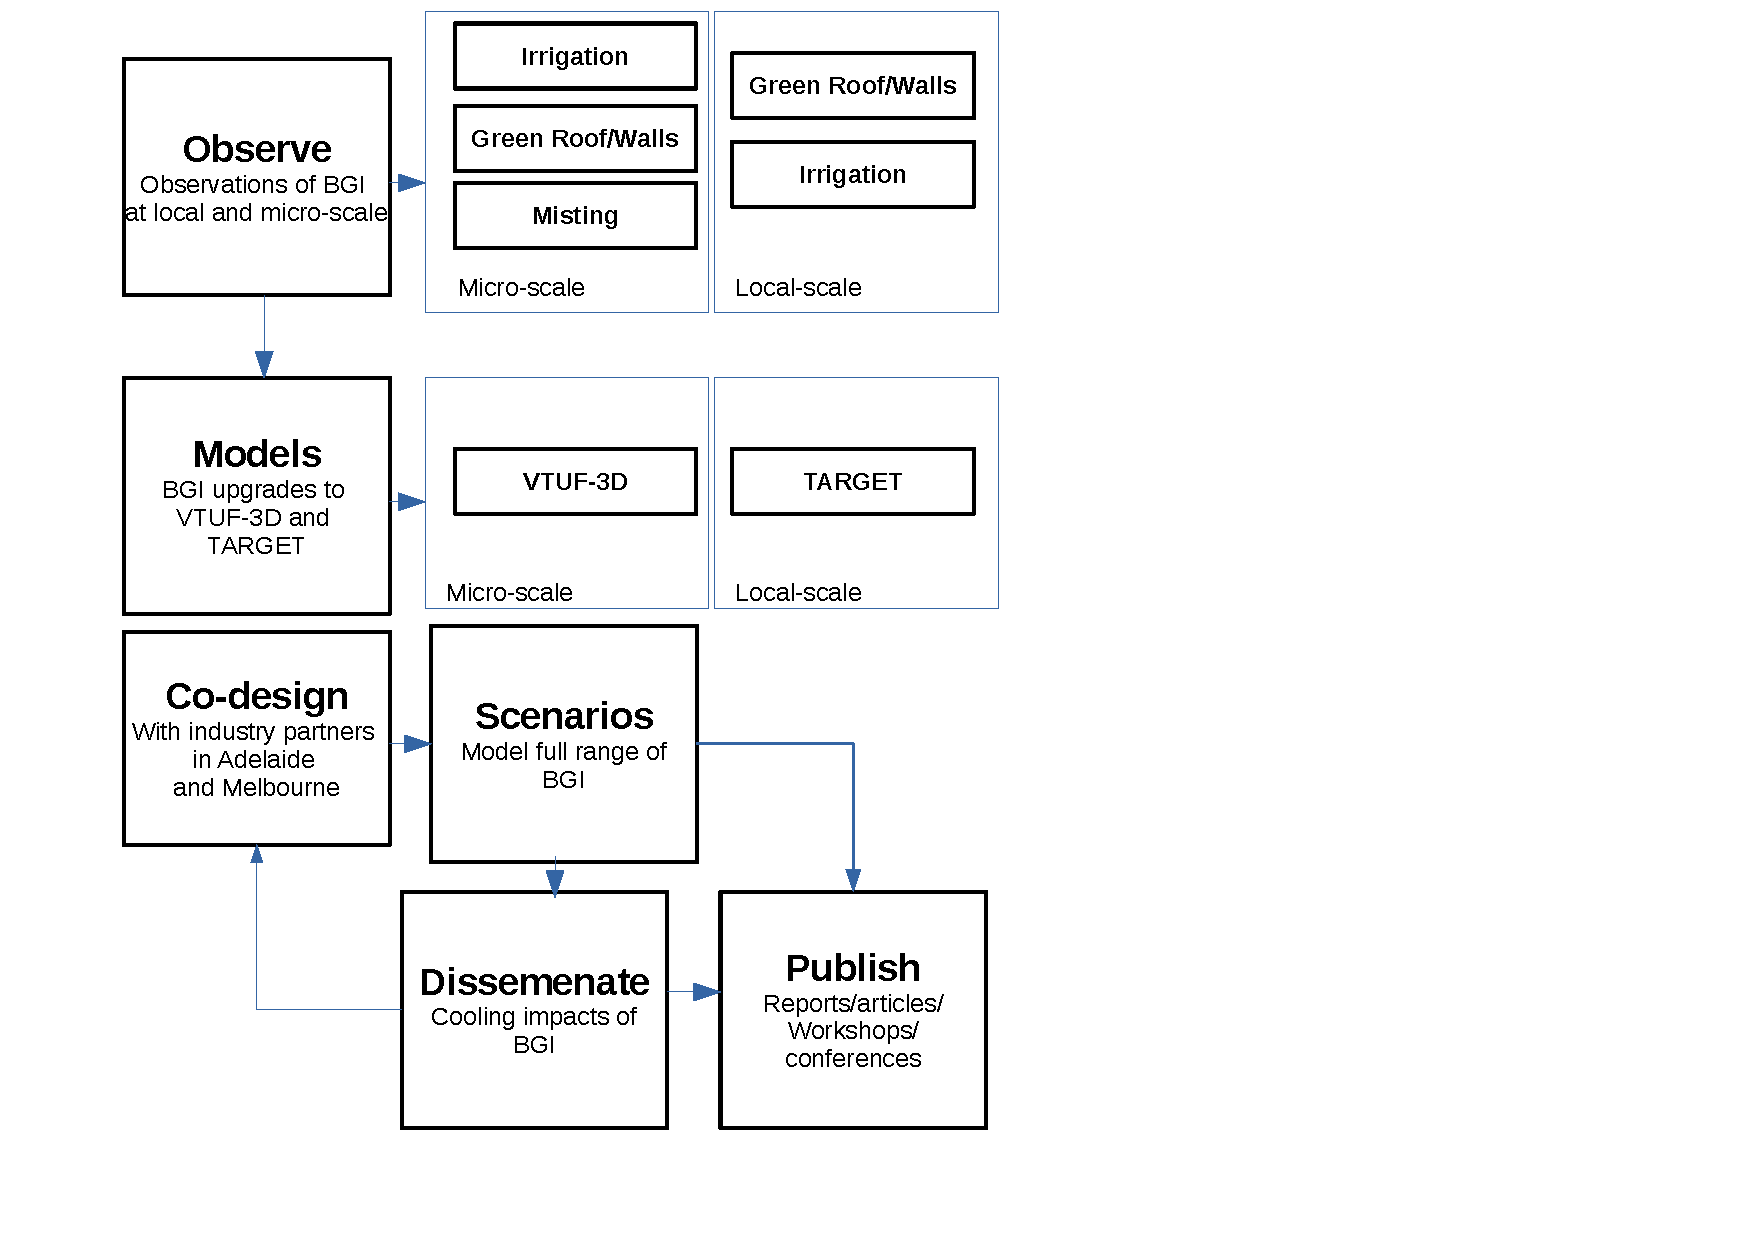
\includegraphics[scale=0.5,trim=40 50 350 0,clip]{Processes.pdf}
}
\end{center}
\caption{Project work packages and steps to achieve urban human thermal comfort analysis of BGI infrastructure.}
\label{fig:overall}
\end{figure}



\textbf{Work Package 1}: \textbf{Observe} - \emph{Collect observations to supply missing datasets needed to parameterise and validate the modelling of the impacts on human thermal comfort of a wide range of BGI types and water usage practices.}

Observations will be made of a range of BGI features at local and micro-scales to enable model development of BGI features. BGI features will include misting systems, green roofs and green walls, and irrigation of vegetated surfaces and impervious surfaces. 

In addition, a number of observations have been made or are currently being collected. At a local scale, misting observations have been collected by Greg Ingleton of South Australia Water. A residential cooling project across Adelaide installed misting system at around 100 residences along with thermometers, flow meters, and soil moisture probes. Surveys have been taken quantifying the effectiveness of the cooling and the impacts on their outdoor behaviour and comfort. Also at a local scale, irrigation trials were conducted within the Adelaide Airport, irrigating a 3.5 hectare site and monitoring the air temperature cooling over a multi-year period\cite{CRCWCS2018,Ingleton2020,Qian2020}. 

Observations at a micro-scale will be captured in 2020-2022, as part of a PhD project, across South East Water's Aquarevo housing estate. Micro-climate and detailed soil property observations (air temperature, humidity, incoming and outgoing shortwave and longwave, wind speed and direction, mean radiant temperature and 3 layers of soil moisture and soil temperature) are  to be captured at two sites. The first site is a control site that will be irrigated on a typical suburban schedule. The second site will be irrigated using a number of scenarios, maintaining the soil moisture, emptying rain tanks before rain storms, and irrigating during high heat events. In addition, micro-scaled observations of energy balances, air temperatures and humidity will be observed within a misting system. Trials of turf grass irrigation will also be conducted at the University of Melbourne Burnley campus, providing micro-scaled observations (temperatures, energy balances, soil moisture) with varying amounts and times of irrigation (i.e. no irrigation, 4mm/day, 8mm/day, and 12/mm day). Finally, micro-climate observations will be collected in 2021-2022, as an honours project, of pavement watering at the Monash campus.

While these observations are good starting points for some of the following model development and validation, future observation campaigns will expand on these to ensure the full range of BGI can be modelled. Micro-scaled green roof observations will be made in the City of Melbourne in conjunction with Dr. Andrea Pianella (University of Melbourne) and A/Prof Sergio Vera (Pontificia Universidad Cat\'{o}lica). 

Aquarevo will also be the site of wider precinct scale observations to observe the cooling effects of outdoor water use. Aquarevo is an ideal site for this as they mandate rainwater capture in rainwater tanks that are also remotely controlled to minimise overflows by releasing water before rainstorms or before heatwaves. In addition, each house is fitted with smart water meters, providing detailed usage measurements for drinking, rainwater, and recycled water sources. These observations provide a unique opportunity to understand the cooling benefits of irrigation across both micro- and local-scales and provide data essential to ensure that models are correctly modelling the influence of irrigation across these scales. 

 All the observation instruments for the micro-climate sites have been purchased through South East Water's funding of the current PhD project at Aquarevo. Some additional equipment has been requested in this project's budget to fill in observation gaps in the local scaled observations.




\textbf{Work Package 2}: \textbf{Models} - \emph{Urban climate modelling tools will be upgraded and shown suitable to model human thermal comfort impacts of BGI and urban water usage.  }

This work package will focus on utilising existing observational datasets and acquiring additional observations and using them to upgrade the two models I have previously developed (VTUF-3D and TARGET) and perform validations that they are suitable to model the human thermal comfort impacts of a wide range of BGI features and practices. While VTUF-3D, as a micro-scale model, is more suitable for modelling BGI, upgrades will be performed on both models. The code upgrades will be very similar and most can be applied to both. In addition, as TARGET runs about 100 times faster than VTUF-3D, it can be used first during an analysis process to make first-order estimates to guide subsequent more detailed modelling.  The tasks required are as follows:

To add additional surface types, I propose to utilise two existing models to add these missing components. The first is MAESPA\cite{Duursma2012} which is a soil-plant-atmosphere model that has been previously coupled by myself with the TUF-3D model\cite{Krayenhoff2007} to create the VTUF-3D\cite{Nice2018a} urban micro-climate model. This coupling provides the hydrology and physiological processes of a single tree, a stand of trees, or vegetated irrigated surface cover (i.e. turf) that are currently parameterised in TARGET. To add additional surface types (deep water, swales, misting fountains, porous and/or watered pavements), modules from a second model will be utilised from the Urban Tethys-Chloris (UT\&C)\cite{Meili2020} (co-developed by myself). This model provides a wide range of urban hydrology processes (interception, ponding, vadose zone dynamics, runoff, and soil hydrology) and plant water and biophysical relations. It also allows modelling of many different arrangements of vegetation within the urban canyon including green roofs and green walls. Upgrades will include a simple horizontal advection scheme. These processes are currently neglected for computational reasons. With the addition of this new scheme, wind direction, wind speed, and terrain features will be used to distribute temperature fluxes to nearby grid cells at the end of each timestep. Interfaces need to be created to run both in a modelling engine. This handles processing the urban design information, designing the modelling domain, enabling forcing the different forcing types. Design coupling of the models as online component to regional climate model to allow micro and local-scaled feedback to drive regional changes. An additional change to upgrade VTUF-3D to version 2 is to update the vegetation/hydrology scheme to run online with the model, either through closer coupling with MAESPA\cite{Duursma2012} or total/partial replacement with modules from UT\&C\cite{Meili2020}. 

\textbf{Work Package 3}: \textbf{Co-design} - \emph{Consult with key stakeholders, especially water companies, to map out the tools and results that will be of highest value to them. }

In this phase of the project, a co-design process will be conducted with industry partners, particularly with South East Water and South Australia Water. I already have an existing working relationship with both. This process will refine the goals and outcomes for the next phase, the scenario modelling, and ensure the research includes scenarios relevant to their needs. Workshops will be held in Adelaide as well as Melbourne. Workshops in Melbourne will not require additional travel. Quarterly online meetings will continue throughout the project to ensure this engagement remains on track. In the final year, workshops in Adelaide and Melbourne will be used to disseminate the findings and plan future collaborations.


\textbf{Work Package 4}: \textbf{Scenarios} \emph{Quantify BGI cooling impacts.  }

This work package will utilise the newly improved modelling tools to systematically test the cooling impacts of BGI. This will uncover optimal scenario parameters, design limitations, and ranked priorities to guide redesign efforts. These interventions might include increasing the street tree canopy cover, modify irrigation rates, or  conversion of driveways and other hard surfaces to permeable pavement. Redesigned areas are iteratively modelled and analysed to converge on the best designs and discover the significant factors impacting urban heat and generate redesigned areas. Additional analysis will allow adding in layers of urban typologies characteristics and demographics to look at the impacts of the heat modelling results on population health.
 
\textbf{Work Package 5}: \textbf{Disseminate} \emph{Share results and methods from the project.  }

The final work package in the project will be used to disseminate the methods and results. This will proceed in a number of different ways. The first will happen through the co-design process of Work Package 3 and the ongoing engagement with industry partners, involving follow-up workshops and reports. The second will be through the traditional academic outputs of journal publications, international and domestic conference presentation, and ongoing collaborations with other urban climate researchers. The final method will be to package the tools, model code, and datasets so that they can be easily adopted by a wide base of users including other researchers and consultants. My current models are freely available and open source, this project will continue this tradition and make the outputs of the project available to all.




\subsection*{\TitleFont BENEFIT}

%Describe the potential benefits including the:
%- new or advanced knowledge resulting from outcomes of the research;
%- economic, commercial, environmental, social and/or cultural benefits for Australia and
%international communities; and
%- potential contribution to capacity in the Australian Government’s National Science and
%Research Priorities and other priorities identified by government.

The fundamental observations of cooling impacts of BGI and the improvements to the models based on these observations will deliver benefits on two levels. The observations will help build our knowledge about how BGI can cool cities and be best used in heat mitigation strategies. The increased sophistication of the models will enable increasingly detailed research to be performed by academic researchers in city science and urban climate. In addition, these modelling tools will help practitioners who need to make immediate decisions about the future design of cities and allow assessments to be made about urban heat mitigation and adaptation strategies using vegetation and the use of water practices. The analysis tools can also be used to examine urban areas for hotspots, areas of high vulnerability, that require immediate attention for remediation to reduce the vulnerability and to provide warning to emergency responders and crisis services for areas that might require extra attention during heat waves. This is work that previously could only be performed using expensive and difficult to obtain observations, often incomplete and captured at only a single point in time.

The 2010s was the hottest decade on record and heatwave occurrences and intensities are projected to be even more frequent in the future. The cost of climate change to society will be especially large in urban areas, while the importance of infrastructure planning and management will grow accordingly. This project, with the aim of contributing to better understanding of urban heat and exploring methods to reducing its impact through data acquisition and model development and validation, will help urban planners and city managers to make better, evidence-based decisions, to design better new cities. It will also support the retrofitting of existing areas and design of new more liveable and climate-safe cities. Climate change will also bring new regional weather patterns and understanding how different areas might perform under these new conditions allows better planning future responses to best protect human health.


% how to achieve impact (benefit outside the academy)
% during project
% at end and immediately after
% over next 2-3 years



The benefits will be achieved over a number of stages. The first benefit is the improved urban climate models. That will happen after the first year and those will be enable those benefits to be used by other researchers. This will be integrated into the research of the THUD research lab, as another component in urban design and health. The second stage of benefits results after integrating the tools into the platform following the second year. This will enable working on case studies with industry collaborators. For example, South East Water, Villawood Properties, and Arden Homes have made large investments in designing and building a sustainable and water and energy efficient housing estate and are very interested in being able to showcase the full range of benefits (including cooling using water) to potential customers and to bring sustainable housing into the mainstream. Finally, after the final delivery of the project, the entire platform will be available to a wide range of users. Urban planners, consultants, property developers, among others will be able to test how, where, how much, and what kind of BGI can be used in urban areas to maximise the cooling benefits and create heat resilient cities. As Australian cities become hotter and denser, populations become more elderly and vulnerable to heat risks, these tools will become increasingly important to plan and react to these growing challenges.

\subsection*{\TitleFont FEASIBILITY}

%Describe the:
%- cost-effectiveness of the research and its value for money;
%- feasibility of the research (including contribution of the project’s design, participants
%and resources to the timely completion of the project);
%- supportive environment for the DECRA candidate and their project, and for HDR
%students where appropriate; and
%- availability of the necessary facilities to complete the project.


While developing climate models is complicated and time consuming, my investigator capability demonstrates that I am the ideal person to develop this project. In addition, many of the micro-climate observations needed for the model development and validation will be provided before and during the first stages of this project through an existing PhD supervised project allowing some of the model development to proceed immediately. Additional local-scaled observations can utilise some of the existing equipment through that research project and through support from South East Water to purchase and install. Additional specialised equipment to supplement these has been requested in the equipment budget in this project. All of these datasets will be unique and have many uses outside of their original projects, especially the ones examining the influence of outdoor irrigation on neighbourhood cooling patterns. These observations have not been possible before, without the detailed water usage data that South East Water can provide through the smart meters they have in place across the neighbourhood. Well designed and unique observation datasets can have a long life and be used in a multitude of other research projects. Coutts et al.\cite{Coutts2007} is a perfect example of such a dataset. Adelaide Airport fieldwork will require travel costs to set up, make observations, and disassemble the equipment while Aquarevo work will be performed locally in Melbourne.

Once the modelling tools are created, they can be used for a wide variety of testing scenarios, both analysis of existing places to find vulnerabilities but also testing new ways to design things. The initial scenario building and analysis process will be focused on Melbourne, Adelaide, and other Australian cities but ultimately the methods and findings are highly transferable to other cities, regions, and countries.

For dissemination, as I have a high professional and academic interest in the ongoing and continual improvements in the modelling tools I have created, they will continue past the end of this project. The code for them will always be available through open repositories (i.e. Github or Bitbucket), made available to the international community of urban climate researchers, and the use and development of them will continue through my academic career. 


Industry engagement, especially with the water companies, through consultation and workshops to work through the scenario designs will require travel to Adelaide in the second and third years and travel is included in the budget. However, the rest of the project will be Melbourne based and not require additional travel budget.

At the University of Melbourne, the Transportation, Health and Urban Design Research Lab was created with multi-year seed funding from the university bringing together a large number of researchers from the Faculty around common research themes. This lab provides a very supportive environment for myself and this research. Much of this research can be undertaken in collaboration with other members of this group, and their expertise in research, particularly in the fields of urban analytics, artificial intelligence, and computer vision, is extremely high. Furthermore, the university provides high levels of support to research facilities, including an extensive high performance computing infrastructure (CPU and GPU) with terabytes of available storage. I have gained extensive experience utilising this resource in my research. 

Master's students recruited by the university are generally high quality and many of them have provided valuable research to a number of my past projects. For example, the supervision of three Master's of IT final semester research projects have resulted in methods that were integrated into my 2020 Urban Climate sky pixels publication\cite{Nice2020}. This method of student supervision is an ideal method to provide research experience to Master's students but also to build capacity and gain assistance with development of small discrete portions of this project. However, to mitigate the risk that these projects might produce useful research but that is not directly related to the goals of this project, a modest amount of hours are allocated across the three years for research assistants. In addition, some additional research assistance will be required throughout the project in data analysis and publication preparation.

The overall project plan and timeline are shown in Figure \ref{fig:timeline}

\begin{figure}[ht]
\centering
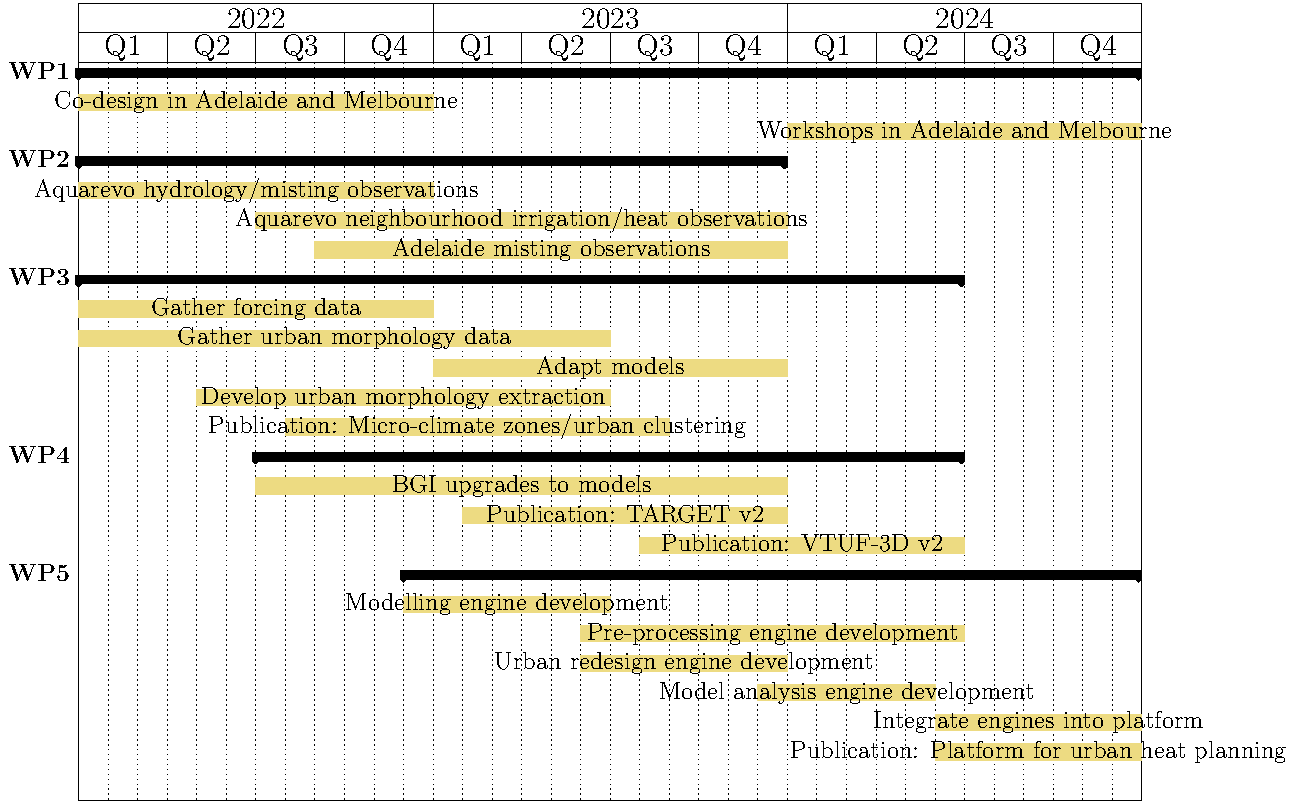
\includegraphics[scale=0.70]{DECRA-D-timeline.pdf}
\caption{Project timeline. }
\label{fig:timeline}
\end{figure}


\subsection*{\TitleFont COMMUNICATION OF RESULTS}

%Outline plans for communicating the research results to other researchers and the broader community, including but not limited to scholarly and public communication and
%dissemination.

There are a number of peer-reviewed publications planned to result from this project (as well as presented at international conferences including ICUC-11, the AMS General Meeting, and the EGU General Assembly). Papers will result from each of the micro and local scaled observations of misting, green roofs, and irrigation. There will be one article each for the upgrade (v2) of the VTUF-3D and TARGET models, to be likely submitted to the Geoscientific Model Development journal. Two additional papers will result from the modelled systematic assessments of BGI at local scales and micro-scales, describing how to use these distinct types of urban design to deliver the best thermal performance under extreme heat conditions and what mitigation strategies work best to reduce the risk in vulnerable areas.

Reports will be written reporting on the overall findings from the project of development designs and mitigation strategies for the industry partners. A project wrap-up will involve a stakeholder workshop with previous partners (for example the City of Melbourne or the Victoria Department of Environment, Land, Water and Planning) to disseminate these reports and help plan the next stages for the research beyond this project.

Beyond academic outputs, translations of the research for more general audiences will be disseminated through platforms such as The Conversation and the University of Melbourne's Pursuit. For example, my recent publication on identifying urban typologies through through the use of urban imagery and computer vision techniques was featured in Pursuit\cite{Nice2020c} and the Sydney Morning Herald\cite{Gladstone2018a}. 

Finally, the models, their code, and observational datasets will be distributed as open-source bundles will allow other interested users to use and extend the work.




\subsection*{\TitleFont REFERENCES}
\renewcommand{\refname}{\normalfont\selectfont\TitleFont REFERENCES} 
\begingroup
\fontsize{10pt}{10pt}\selectfont
\bibliographystyle{abbrv}


\bibliography{library2}



%Include a list of all references, including relevant references to the previous work of the candidate. References may be in 10 point font.






%\end{document}
